\documentclass[12pt,a4paper]{article}

% Packages
\usepackage{geometry}
\geometry{margin=1in}
\usepackage{fancyhdr}
\usepackage{titlesec}
\usepackage{listings}
\usepackage{xcolor}
\usepackage{graphicx}

% Header & Footer
\pagestyle{fancy}
\fancyhf{}
\rhead{DBT - Assignment 5}
\lhead{Kamithkar Vinod}
\cfoot{\thepage}

% Title formatting
\titleformat{\section}{\large\bfseries}{Problem \thesection:}{0.5em}{}
\titleformat{\subsection}[runin]{\bfseries}{Code:}{0.5em}{}[---]
\titleformat{\subsubsection}[runin]{\bfseries}{Output:}{0.5em}{}[---]

% SQL language definition for listings
\lstdefinelanguage{SQL}{
  morekeywords={
    SELECT, FROM, WHERE, GROUP, BY, ORDER, ASC, DESC, JOIN, ON, AS,
    AND, OR, NOT, IN, IS, NULL, LIKE, HAVING, COUNT, SUM, AVG, MIN, MAX,
    CREATE, TABLE, INSERT, INTO, VALUES, UPDATE, SET, DELETE, DISTINCT,
    CASE, WHEN, THEN, ELSE, END, BETWEEN, EXISTS, UNION, ALL, ANY, LEFT,
    RIGHT, INNER, OUTER, LIMIT, OFFSET, PROCEDURE, BEGIN, FUNCTION, END, RETURNS, RETURN
  },
  sensitive=false,
  morecomment=[l]{--},
  morestring=[b]',
}

\lstset{
    language=SQL,
    basicstyle=\ttfamily\small,
    keywordstyle=\color{blue}\bfseries,
    commentstyle=\color{gray}\itshape,
    stringstyle=\color{red},
    showstringspaces=false,
    frame=single,
    breaklines=true,
    numbers=none
}

% Document Start
\begin{document}

% Title Page
\begin{center}
    \LARGE \textbf{Assignment - 5} \\[0.5cm]
    \Large \textbf{DBMS} \\[1cm]

    \begin{tabular}{rl}
        \textbf{Name:} & Kamithkar Vinod \\
        \textbf{Course:} & PG DAC AUGUST 2025 \\
        \textbf{PRN:} & 250850320040 \\
        \textbf{Form No:} & 250500480 \\
        \textbf{Date:} & 28-10-2025 \\
    \end{tabular}
\end{center}

\vspace{1cm}
\hrule
\vspace{0.5cm}

% Problems

% 1
\section{LOOP}
\textbf{Task:} Increase salary of first 3 employees by 10%.

\subsection{}
\begin{lstlisting}
drop procedure if exists loop_increase_salary;

delimiter //
create procedure loop_increase_salary() 
begin
    declare i int default 1;
    declare total int;

    select count(*) into total from employees;

    loop_label: loop
        if i > 3 then
            leave loop_label;
        end if;

        update employees set salary = salary * 1.10 where id = i;
        set i = i + 1;
    end loop loop_label;
end //
delimiter ;

call loop_increase_salary();

select * from employees;


\end{lstlisting}

\subsubsection{}
\begin{center}
    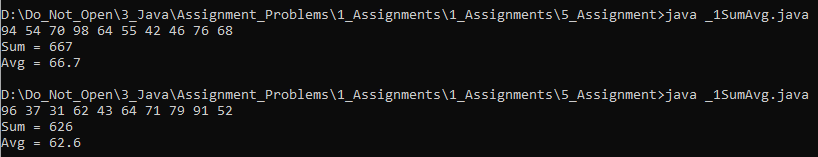
\includegraphics[width=0.8\textwidth]{1.png}
\end{center}

% 2

\section{LOOP}
\textbf{Task:} Display all employee names using LOOP.

\subsection{}
\begin{lstlisting}
DROP PROCEDURE IF EXISTS loop_display_names;
DELIMITER //
CREATE PROCEDURE loop_display_names()
BEGIN
   DECLARE i INT DEFAULT 1;
   DECLARE total INT;
   DECLARE emp_name VARCHAR(50);
   SELECT COUNT(*) INTO total FROM employees;

   display_loop: LOOP
       IF i > total THEN
           LEAVE display_loop;
       END IF;
       SELECT name INTO emp_name FROM employees WHERE id = i;
       SELECT emp_name AS Employee_Name;
       SET i = i + 1;
   END LOOP display_loop;
END //
DELIMITER ;
CALL loop_display_names();


\end{lstlisting}

\subsubsection{}
\begin{center}
    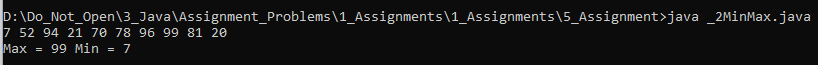
\includegraphics[width=0.8\textwidth]{2.png}
\end{center}

% 3

\section{LOOP}
\textbf{Task:} Calculate total salary of all employees using LOOP.

\subsection{}
\begin{lstlisting}
DROP PROCEDURE IF EXISTS loop_total_salary;
DELIMITER //
CREATE PROCEDURE loop_total_salary()
BEGIN
   DECLARE i INT DEFAULT 1;
   DECLARE total INT;
   DECLARE total_salary DECIMAL(10,2) DEFAULT 0;
   DECLARE sal DECIMAL(10,2);
   SELECT COUNT(*) INTO total FROM employees;

   salary_loop: LOOP
       IF i > total THEN
           LEAVE salary_loop;
       END IF;
       SELECT salary INTO sal FROM employees WHERE id = i;
       SET total_salary = total_salary + sal;
       SET i = i + 1;
   END LOOP salary_loop;
   SELECT total_salary AS Total_Salary;
END //
DELIMITER ;
CALL loop_total_salary();

\end{lstlisting}

\subsubsection{}
\begin{center}
    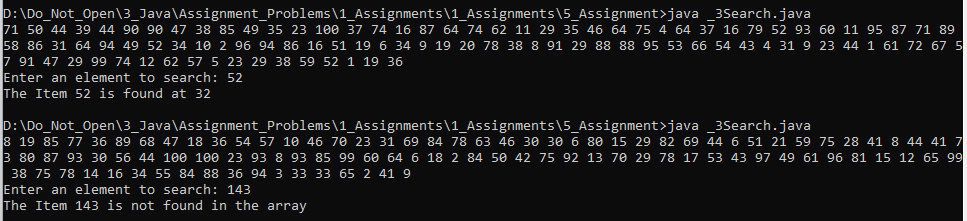
\includegraphics[width=0.8\textwidth]{3.png}
\end{center}

% 4

\section{LOOP}
\textbf{Task:} Insert 3 new temporary employees into the table using LOOP.

\subsection{}
\begin{lstlisting}
DROP PROCEDURE IF EXISTS loop_insert_temps;
DELIMITER //
CREATE PROCEDURE loop_insert_temps()
BEGIN
   DECLARE i INT DEFAULT 1;
   temp_loop: LOOP
       IF i > 3 THEN
           LEAVE temp_loop;
       END IF;
	INSERT INTO employees(name, department, salary)
       VALUES (CONCAT('TempEmp', i), 'Temp', 20000);
       SET i = i + 1;
   END LOOP temp_loop;
END //
DELIMITER ;
CALL loop_insert_temps();
SELECT * FROM employees;

\end{lstlisting}

\subsubsection{}
\begin{center}
    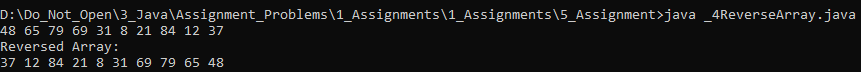
\includegraphics[width=0.8\textwidth]{4.png}
\end{center}

% 5

\section{LOOP}
\textbf{Task:} Display employee names department-wise using LOOP.
Loop through all departments and show employee names under each.

\subsection{}
\begin{lstlisting}
DROP PROCEDURE IF EXISTS loop_names_by_department;
DELIMITER //
CREATE PROCEDURE loop_names_by_department()
BEGIN
  DECLARE i INT DEFAULT 1;
  DECLARE total INT;
  DECLARE dept VARCHAR(30);
  DECLARE emp_name VARCHAR(50);
  SELECT COUNT(*) INTO total FROM employees;

  loop_label: LOOP
      IF i > total THEN
          LEAVE loop_label;
      END IF;
      SELECT department, name INTO dept, emp_name FROM employees WHERE id = i;
      SELECT CONCAT('Department: ', dept, ' - ', emp_name) AS Employee_Info;
      SET i = i + 1;
  END LOOP loop_label;
END //
DELIMITER ;
CALL loop_names_by_department();

\end{lstlisting}

\subsubsection{}
\begin{center}
    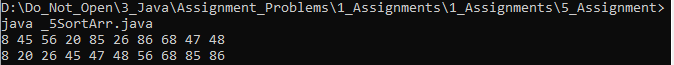
\includegraphics[width=0.8\textwidth]{5.png}
\end{center}

% 6

\section{LOOP}
\textbf{Task:} Grant a ₹2,000 performance bonus to each IT department employee using
LOOP.
Traverse through each employee and update if the department is ‘IT’.

\subsection{}
\begin{lstlisting}
DROP PROCEDURE IF EXISTS loop_bonus_it;
DELIMITER //
CREATE PROCEDURE loop_bonus_it()
BEGIN
  DECLARE i INT DEFAULT 1;
  DECLARE total INT;
  DECLARE dept VARCHAR(30);
  SELECT COUNT(*) INTO total FROM employees;

  bonus_loop: LOOP
      IF i > total THEN
          LEAVE bonus_loop;
      END IF;
      SELECT department INTO dept FROM employees WHERE id = i;
      IF dept = 'IT' THEN
          UPDATE employees SET salary = salary + 2000 WHERE id = i;
      END IF;
      SET i = i + 1;
  END LOOP bonus_loop;
END //
DELIMITER ;
CALL loop_bonus_it();
SELECT * FROM employees;

\end{lstlisting}

\subsubsection{}
\begin{center}
    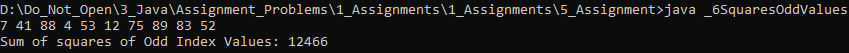
\includegraphics[width=0.8\textwidth]{6.png}
\end{center}

% 7

\section{LOOP}
\textbf{Task:} Find and display the highest salary among all employees using LOOP.

\subsection{}
\begin{lstlisting}
DROP PROCEDURE IF EXISTS loop_highest_salary;
DELIMITER //
CREATE PROCEDURE loop_highest_salary()
BEGIN
  DECLARE i INT DEFAULT 1;
  DECLARE total INT;
  DECLARE sal DECIMAL(10,2);
  DECLARE max_sal DECIMAL(10,2) DEFAULT 0;
  SELECT COUNT(*) INTO total FROM employees;

  find_loop: LOOP
      IF i > total THEN
          LEAVE find_loop;
	END IF;
		  SELECT salary INTO sal FROM employees WHERE id = i;
		  IF sal > max_sal THEN
			  SET max_sal = sal;
		  END IF;
		  SET i = i + 1;
	  END LOOP find_loop;
	  SELECT max_sal AS Highest_Salary;
END //
DELIMITER ;
CALL loop_highest_salary();

\end{lstlisting}

\subsubsection{}
\begin{center}
    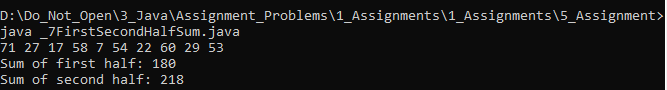
\includegraphics[width=0.8\textwidth]{7.png}
\end{center}

% 8

\section{LOOP}
\textbf{Task:} Copy data of first 2 employees into a new table employee_backup using LOOP.

\subsection{}
\begin{lstlisting}
DROP PROCEDURE IF EXISTS loop_copy_to_backup;
DELIMITER //
CREATE PROCEDURE loop_copy_to_backup()
BEGIN
  DECLARE i INT DEFAULT 1;
  CREATE TABLE IF NOT EXISTS employee_backup LIKE employees;

  copy_loop: LOOP
      IF i > 2 THEN
          LEAVE copy_loop;
      END IF;
      INSERT INTO employee_backup(name, department, salary)
      SELECT name, department, salary FROM employees WHERE id = i;
      SET i = i + 1;
  END LOOP copy_loop;
END //
DELIMITER ;
CALL loop_copy_to_backup();
SELECT * FROM employee_backup;

\end{lstlisting}

\subsubsection{}
\begin{center}
    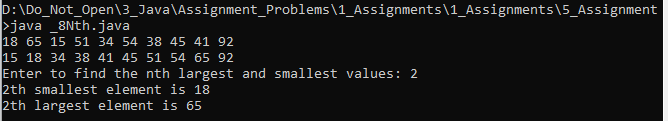
\includegraphics[width=0.8\textwidth]{8.png}
\end{center}

% 9

\section{WHILE}
\textbf{Task:} Display employees having salary greater than ₹30,000.

\subsection{}
\begin{lstlisting}
DROP PROCEDURE IF EXISTS while_high_salary;
DELIMITER //
CREATE PROCEDURE while_high_salary()
BEGIN
   DECLARE i INT DEFAULT 1;
   DECLARE total INT;
   DECLARE sal DECIMAL(10,2);
   DECLARE emp_name VARCHAR(50);
   SELECT COUNT(*) INTO total FROM employees;

   WHILE i <= total DO
       SELECT salary, name INTO sal, emp_name FROM employees WHERE id = i LIMIT 1;
       IF sal > 30000 THEN
           SELECT emp_name AS Name, sal AS Salary;
       END IF;
       SET i = i + 1;
   END WHILE;
END //
DELIMITER ;
CALL while_high_salary();

\end{lstlisting}

\subsubsection{}
\begin{center}
    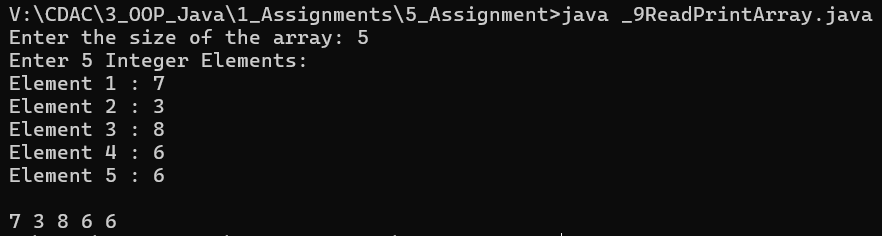
\includegraphics[width=0.8\textwidth]{9.png}
\end{center}

% 10

\section{WHILE}
\textbf{Task:} Increase one employee’s salary incrementally by 5000 until it reaches ₹50,000.

\subsection{}
\begin{lstlisting}
DROP PROCEDURE IF EXISTS while_increase_until;
DELIMITER //
CREATE PROCEDURE while_increase_until()
BEGIN
	DECLARE sal DECIMAL(10,2);
	DECLARE emp_name VARCHAR(50);
	SELECT salary, name INTO sal, emp_name FROM employees WHERE id = 1;
	WHILE sal < 50000 DO
	   SET sal = sal + 5000;
	   SELECT CONCAT(emp_name, ' salary increased to ', sal) AS Progress;
	END WHILE;
END //
DELIMITER ;
CALL while_increase_until();

\end{lstlisting}

\subsubsection{}
\begin{center}
    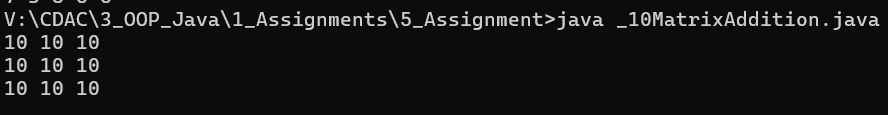
\includegraphics[width=0.8\textwidth]{10.png}
\end{center}

% 11

\section{WHILE}
\textbf{Task:} Count total IT department employees.

\subsection{}
\begin{lstlisting}
DROP PROCEDURE IF EXISTS while_count_it;
DELIMITER //
CREATE PROCEDURE while_count_it()
BEGIN
   DECLARE i INT DEFAULT 1;
   DECLARE total INT;
   DECLARE dept VARCHAR(30);
   DECLARE count_it INT DEFAULT 0;
   SELECT COUNT(*) INTO total FROM employees;

   WHILE i <= total DO
       SELECT department INTO dept FROM employees WHERE id = i;
       IF dept = 'IT' THEN
           SET count_it = count_it + 1;
       END IF;
       SET i = i + 1;
   END WHILE;
   SELECT count_it AS Total_IT_Employees;
END //
DELIMITER ;
CALL while_count_it();

\end{lstlisting}

\subsubsection{}
\begin{center}
    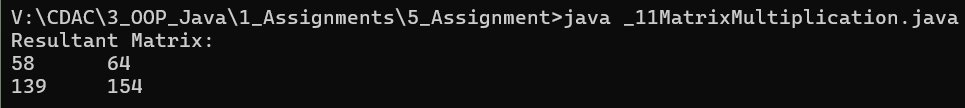
\includegraphics[width=0.8\textwidth]{11.png}
\end{center}

% 12

\section{WHILE}
\textbf{Task:} Display employees whose name length is less than 6 characters using WHILE.

\subsection{}
\begin{lstlisting}
DROP PROCEDURE IF EXISTS while_short_names;
DELIMITER //
CREATE PROCEDURE while_short_names()
BEGIN
  DECLARE i INT DEFAULT 1;
  DECLARE total INT;
  DECLARE emp_name VARCHAR(50);
  SELECT COUNT(*) INTO total FROM employees;

  WHILE i <= total DO
      SELECT name INTO emp_name FROM employees WHERE id = i;
      IF CHAR_LENGTH(emp_name) < 6 THEN
          SELECT emp_name AS Short_Name;
      END IF;
      SET i = i + 1;
  END WHILE;
END //
DELIMITER ;
CALL while_short_names();

\end{lstlisting}

\subsubsection{}
\begin{center}
    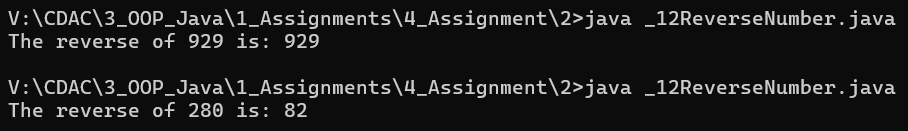
\includegraphics[width=0.8\textwidth]{12.png}
\end{center}

% 13

\section{WHILE}
\textbf{Task:} Deduct ₹1,000 from one employee’s salary until it reaches ₹25,000 using
WHILE.

\subsection{}
\begin{lstlisting}
DROP PROCEDURE IF EXISTS while_deduct_salary;
DELIMITER //
CREATE PROCEDURE while_deduct_salary()
BEGIN
  DECLARE sal DECIMAL(10,2);
  DECLARE emp_name VARCHAR(50);
  SELECT salary, name INTO sal, emp_name FROM employees WHERE id = 3;

  WHILE sal > 25000 DO
      SET sal = sal - 1000;
      SELECT CONCAT(emp_name, ' salary reduced to ', sal) AS Progress;
  END WHILE;
END //
DELIMITER ;
CALL while_deduct_salary();

\end{lstlisting}

\subsubsection{}
\begin{center}
    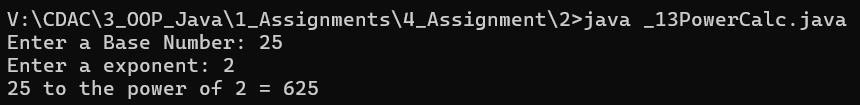
\includegraphics[width=0.8\textwidth]{13.png}
\end{center}

% 14

\section{WHILE}
\textbf{Task:} Calculate average salary of all employees using WHILE.

\subsection{}
\begin{lstlisting}
DROP PROCEDURE IF EXISTS while_average_salary;
DELIMITER //
CREATE PROCEDURE while_average_salary()
BEGIN
  DECLARE i INT DEFAULT 1;
  DECLARE total INT;
  DECLARE total_sal DECIMAL(10,2) DEFAULT 0;
  DECLARE sal DECIMAL(10,2);
  SELECT COUNT(*) INTO total FROM employees;

  WHILE i <= total DO
      SELECT salary INTO sal FROM employees WHERE id = i;
      SET total_sal = total_sal + sal;
      SET i = i + 1;
  END WHILE;
  SELECT (total_sal / total) AS Average_Salary;
END //
DELIMITER ;
CALL while_average_salary();

\end{lstlisting}

\subsubsection{}
\begin{center}
    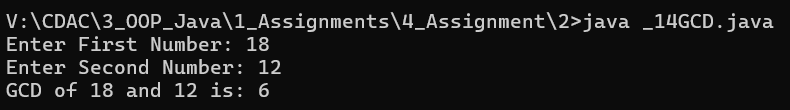
\includegraphics[width=0.8\textwidth]{14.png}
\end{center}

% 15

\section{REPEAT}
\textbf{Task:} Add ₹5,000 to one employee’s salary until it exceeds ₹40,000.

\subsection{}
\begin{lstlisting}
DROP PROCEDURE IF EXISTS repeat_add_salary;
DELIMITER //
CREATE PROCEDURE repeat_add_salary()
BEGIN
   DECLARE sal DECIMAL(10,2);
   DECLARE emp_name VARCHAR(50);
   SELECT salary, name INTO sal, emp_name FROM employees WHERE id = 2;
   REPEAT
       SET sal = sal + 5000;
       SELECT CONCAT('New salary of ', emp_name, ' is ', sal) AS Info;
   UNTIL sal > 40000
   END REPEAT;
END //
DELIMITER ;
CALL repeat_add_salary();

\end{lstlisting}

\subsubsection{}
\begin{center}
    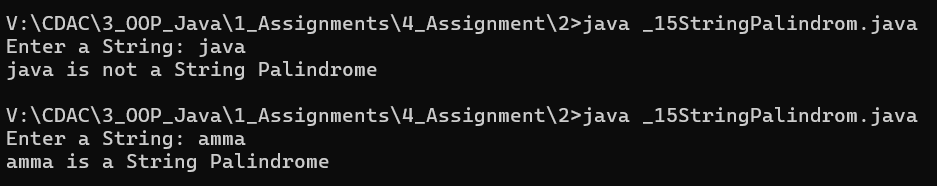
\includegraphics[width=0.8\textwidth]{15.png}
\end{center}

% 16

\section{REPEAT}
\textbf{Task:} Insert employees until 10 total records exist.

\subsection{}
\begin{lstlisting}
DROP PROCEDURE IF EXISTS repeat_insert_until10;
DELIMITER //
CREATE PROCEDURE repeat_insert_until10()
BEGIN
   DECLARE total INT;
   SELECT COUNT(*) INTO total FROM employees;
   REPEAT
       INSERT INTO employees(name, department, salary)
       VALUES (CONCAT('ExtraEmp', total + 1), 'Support', 25000);
       SELECT COUNT(*) INTO total FROM employees;
   UNTIL total >= 10
   END REPEAT;
END //
DELIMITER ;
CALL repeat_insert_until10();
SELECT * FROM employees;

\end{lstlisting}

\subsubsection{}
\begin{center}
    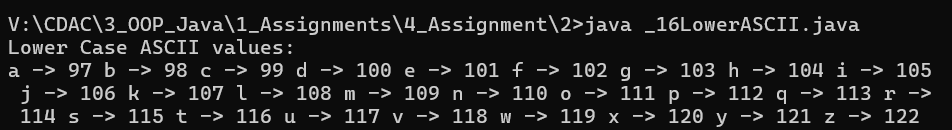
\includegraphics[width=0.8\textwidth]{16.png}
\end{center}

% 17

\section{REPEAT}
\textbf{Task:} Keep adding bonuses until total crosses ₹1,00,000.

\subsection{}
\begin{lstlisting}
DROP PROCEDURE IF EXISTS repeat_bonus_pool;
DELIMITER //
CREATE PROCEDURE repeat_bonus_pool()
BEGIN
   DECLARE total_bonus DECIMAL(10,2) DEFAULT 0;
   DECLARE bonus DECIMAL(10,2) DEFAULT 15000;
   REPEAT
       SET total_bonus = total_bonus + bonus;
       SELECT total_bonus AS Current_Bonus;
   UNTIL total_bonus > 100000
   END REPEAT;
END //
DELIMITER ;
CALL repeat_bonus_pool();

\end{lstlisting}

\subsubsection{}
\begin{center}
    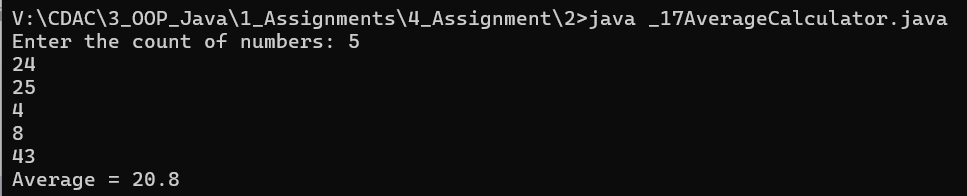
\includegraphics[width=0.8\textwidth]{17.png}
\end{center}

% 18

\section{REPEAT}
\textbf{Task:} Keep inserting random temporary employees until 15 total employees exist
using REPEAT.

\subsection{}
\begin{lstlisting}
DROP PROCEDURE IF EXISTS repeat_insert_until15;
DELIMITER //
CREATE PROCEDURE repeat_insert_until15()
BEGIN
  DECLARE total INT;
  SELECT COUNT(*) INTO total FROM employees;
  REPEAT
      INSERT INTO employees(name, department, salary)
      VALUES (CONCAT('TempEmp', total + 1), 'Support', 22000);
      SELECT COUNT(*) INTO total FROM employees;
  UNTIL total >= 15
  END REPEAT;
END //
DELIMITER ;
CALL repeat_insert_until15();
SELECT * FROM employees;

\end{lstlisting}

\subsubsection{}
\begin{center}
    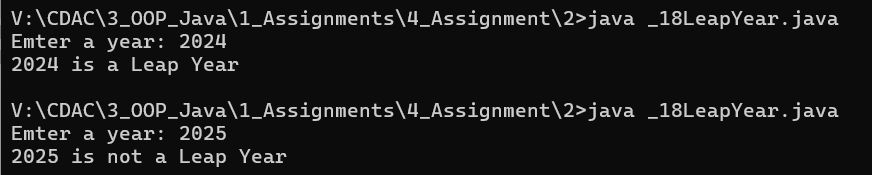
\includegraphics[width=0.8\textwidth]{18.png}
\end{center}

% 19

\section{REPEAT}
\textbf{Task:} Keep adding ₹500 increments to a specific employee’s salary until it reaches
₹45,000 using REPEAT.

\subsection{}
\begin{lstlisting}
DROP PROCEDURE IF EXISTS repeat_raise_salary;
DELIMITER //
CREATE PROCEDURE repeat_raise_salary()
BEGIN
  DECLARE sal DECIMAL(10,2);
  DECLARE emp_name VARCHAR(50);
  SELECT salary, name INTO sal, emp_name FROM employees WHERE id = 4;
  REPEAT
      SET sal = sal + 500;
      SELECT CONCAT('Salary of ', emp_name, ' is now ', sal) AS UpdateInfo;
  UNTIL sal >= 45000
  END REPEAT;
END //
DELIMITER ;
CALL repeat_raise_salary();

\end{lstlisting}

\subsubsection{}
\begin{center}
    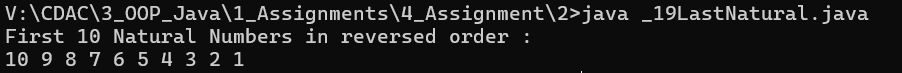
\includegraphics[width=0.8\textwidth]{19.png}
\end{center}

% 20

\section{REPEAT}
\textbf{Task:} Display employee salaries one by one using REPEAT until all records are printed.

\subsection{}
\begin{lstlisting}
DROP PROCEDURE IF EXISTS repeat_display_salaries;
DELIMITER //
CREATE PROCEDURE repeat_display_salaries()
BEGIN
  DECLARE i INT DEFAULT 1;
  DECLARE total INT;
  DECLARE emp_name VARCHAR(50);
  DECLARE sal DECIMAL(10,2);
  SELECT COUNT(*) INTO total FROM employees;

  REPEAT
      SELECT name, salary INTO emp_name, sal FROM employees WHERE id = i;
      SELECT CONCAT(emp_name, ' earns ₹', sal) AS Employee_Salary;
      SET i = i + 1;
  UNTIL i > total
  END REPEAT;
END //
DELIMITER ;
CALL repeat_display_salaries();

\end{lstlisting}

\subsubsection{}
\begin{center}
    
\includegraphics[width=0.8\textwidth]{20.png}
\end{center}

\end{document}
